\chapter{Transformer models}
\label{chap:transformers}

\begin{supportbox}{About this chapter}
Convolutional models are strong baselines, especially for images and sequences where local relations prevail, but they are limited in handling very long sequences or non-local dependencies between elements of a sequence. In this chapter we introduce another class of models, called transformers, which are designed to overcome such challenges.
\end{supportbox}

\section{Long convolutions and non-local models}

After the key developments in the period 2012-2016, discussed in the previous chapter, the next important breakthrough in the design of differentiable models came in 2016-2017 with the popularization of the \textbf{transformer} \cite{vaswani2017attention}, an architecture designed to handle efficiently long-range dependencies in natural language processing. Due to its strong scaling laws, the architecture was then extended to other types of data, from images to time-series and graphs, and it is today a state-of-the-art model in many fields due to its very good scaling laws when trained on large amounts of data \cite{kaplan2020scaling,bordes2024introduction}. 

As we will see, an interesting aspect of the transformer is a decoupling between the data type (through the use of appropriate tokenizers) and the architecture, which for the most part remains data-agnostic. This opens up several interesting directions, such as simple multimodal architectures and transfer learning strategies. We begin by motivating the core component of the transformer, called the \textbf{multi-head attention} (MHA) layer. We will defer a discussion on the original transformer model from \cite{vaswani2017attention} to the next chapter.


\begin{supportbox}{A bit of history}
Historically, this chapter is out of order: in 2015, the most common alternative to CNNs for text were \textbf{recurrent neural networks} (RNNs). As an isolated component, MHA was introduced for RNNs \cite{bahdanau2014neural}, before being used as the core component in the transformer model. We cover RNNs and their modern incarnation, linearized RNNs, in Chapter \ref{chap:rnns}. Recently, RNNs have become an attractive competitor to transformers for language modeling.
\end{supportbox}

\subsection{Handling long-range and sparse dependencies}

Consider these two sentences: 
%
\begin{quote}
“\textit{The {\color{drawred}cat} is on the {\color{drawgreen}table}}”
\end{quote}
%
and a longer one:
%
\begin{quote}
“\textit{The {\color{drawred}cat}, who belongs to my mother, is on the {\color{drawgreen}table}}”.
\end{quote}
%
In order to be processed by a differentiable model, the sentences must be tokenized and the tokens embedded as vectors (Chapter \ref{chap:convolutions_beyond_images}). From a semantic point of view, the tokens belonging to the red word ({\color{drawred}cat}) and to the green word ({\color{drawgreen}table}) share a similar dependency in both sentences. However, their relative offset varies in the two cases, and their distance can become arbitrarily large. Hence, dependencies in text can be both \textbf{long-range} and \textbf{input-dependent}.

Denote by $\mathbf{X} \sim (n, e)$ a sentence of $n$ tokens embedded in $e$-dimensional vectors and denote by $\mathbf{x}_i$ the $i$th token. We can rewrite a 1D convolution with kernel size $k$ on token $i$ as follows:
%
\begin{equation}
\mathbf{h}_i=\sum_{j=1}^{2k+1}\mathbf{W}_j \mathbf{x}_{i+k+1-j}
\label{eq:conv_1d}
\end{equation}
%
Each token inside the receptive field is processed with a fixed weight matrix $\mathbf{W}_i$ that only depends on the specific offset $i$. Modeling long-range dependencies inside the layer requires us to increase the receptive field of the layer, increasing the number of parameters linearly in the receptive field. 

\begin{figure}[t]
    \centering
    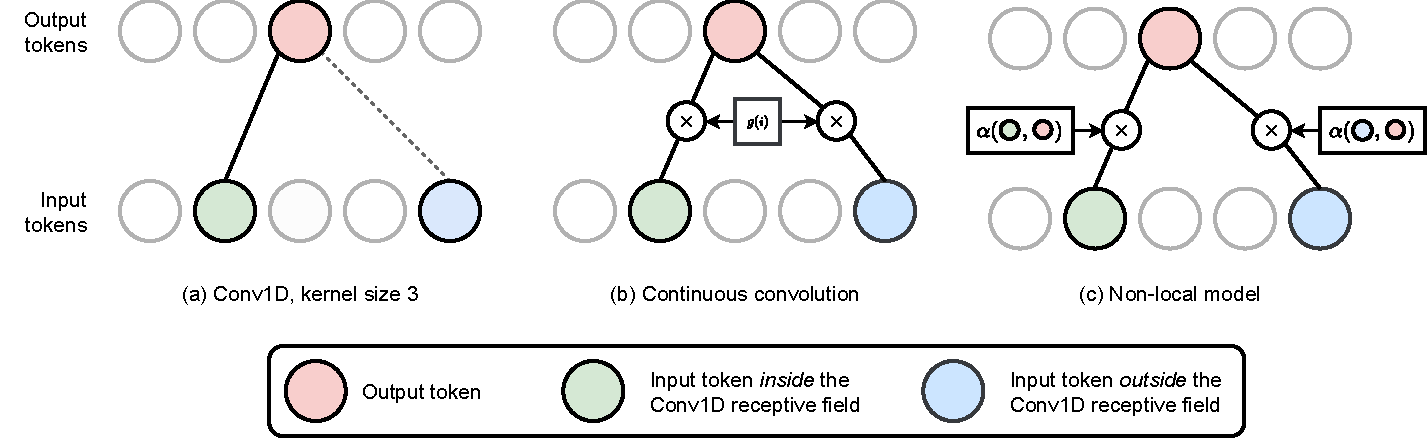
\includegraphics[width=1.0\textwidth]{images/convolution_types}
    \caption{Comparison between different types of convolution for a 1D sequence. We show how one output token (in \colorbox{drawred!30}{red}) interacts with two tokens, one inside the receptive field of the convolution (in \colorbox{drawgreen!30}{green}), and one outside (in \colorbox{drawblue!30}{blue}). (a) In a standard convolution, the blue token is ignored because it is outside of the receptive field of the filter. (b) For a continuous convolution, both tokens are considered, and the resulting weight matrices are given by $g(-1)$ and $g(2)$ respectively. (c) In the non-local case, the weight matrices depend on a pairwise comparison between the tokens themselves.}
    \label{fig:biases}
\end{figure}


One possibility to solve this is the following: instead of explicitly learning the parameter matrices $\mathbf{W}_1, \mathbf{W}_2, \ldots$, we can define them \textit{implicitly} by defining a separate neural block $g(i): \mathbb{R} \rightarrow \mathbb{R}^{e \times e}$ that outputs all weight matrices based on the relative offset $i$. Hence, we rewrite \eqref{eq:conv_1d} as:

$$
\mathbf{h}_i=\eqnmarkbox[drawred]{node}{\sum_{j=1}^n} g(i-j)\mathbf{x}_j
$$
\annotate[yshift=-1em]{below,right}{node}{The sum is now on \textit{all} tokens}

\vspace{1em}
This is called a \textbf{long convolution}, as the convolution spans the entire input matrix $\mathbf{X}$. It is also called a \textbf{continuous convolution} \cite{romero2022towards}, because we can use $g(\cdot)$ to parameterize intermediate positions or variable resolutions \cite{romero2022towards}. The number of parameters in this case only depends on the parameters of $g$, while it does not depend on $n$, the length of the sequence. Defining $g$ is non-trivial because it needs to output an entire weight matrix. We can recover a standard convolution easily:
%
\begin{equation}
    g(i, j) = \begin{cases} \mathbf{W}_{i-j} & \text{ if } \lvert i - j \rvert \le k \\ 0 & \text{ otherwise } \end{cases}
\end{equation}
%
This partially solves the problem of long-range dependencies, but it does not solve the problem of dependencies which are conditional on the input, since the weight given to a token depends only on the relative offset with respect to the index $i$. However, this formulation provides a simple way to tackle this problem by letting the trained function $g$ depend on the \textit{content} of the tokens instead of their positions:
%
\begin{equation}
\mathbf{h}_i=\sum_{j=1}^n {\color{drawred}g(\mathbf{x}_i, \mathbf{x}_j)}\mathbf{x}_j
\label{eq:nonlocal_convolution}
\end{equation}
%
In the context of computer vision, these models are also called \textbf{non-local} networks \cite{wang2018non}. We provide a comparison of standard convolutions, continuous convolutions, and non-local convolutions in Figure \ref{fig:biases}.

\subsection{The attention layer} \addclock

The MHA layer is a simplification of \eqref{eq:nonlocal_convolution}. First, working with functions having matrix outputs is difficult, so we restrict the layer to work with scalar weights. In particular, a simple measure of similarity between tokens is their \textbf{dot-product}:
%
$$
g(\mathbf{x}_i, \mathbf{x}_j)=\mathbf{x}_i^\top\mathbf{x}_j
$$
%
As we will see, this results in an easily parallelizable algorithm for the entire sequence. For the following we consider a normalized version of the dot-product:
%
$$
g(\mathbf{x}_i, \mathbf{x}_j)=\frac{1}{\sqrt{e}}\mathbf{x}_i^\top\mathbf{x}_j
$$
%
This can be motivated as follows: if we assume $\mathbf{x}_i \sim \mathcal{N}(0, \sigma^2\mathbf{I})$, the variance of each element of $\mathbf{x}_i^\top\mathbf{x}_j$ is $\sigma^4$, hence the elements can easily grow very large in magnitude. The scaling factor ensures that the variance of the dot product remains bounded at $\sigma^2$.

Because we are summing over a potentially variable number of tokens $n$, it is also helpful to include a normalization operation, such as a softmax:\footnote{The notation $\text{softmax}_j$ in \eqref{eq:pre_self_attention} means we are applying the softmax normalization to the set $\left\{g(\mathbf{x}_i, \mathbf{x}_j)\right\}_{j=1}^n$, independently for each $i$. This is easier to see in the vectorized case, described below.}
%
\begin{equation}
\mathbf{h}_i=\sum_{j=1}^n {\color{drawgreen}\text{softmax}_j}(g(\mathbf{x}_i, \mathbf{x}_j))\mathbf{x}_j
\label{eq:pre_self_attention}
\end{equation}

In this context, we refer to $g(\cdot, \cdot)$ as the \textbf{attention scoring function}, and to the output of the softmax as the \textbf{attention scores}. Because of the normalization properties of the softmax, we can imagine that each token $i$ has a certain amount of “attention” it can allocate across the other tokens: by increasing the budget on a token, the attention over the other tokens will necessarily decrease due to the denominator in the softmax.

\vspace{-0.5em}
If we use a “dot-product attention”, our $g$ does not have trainable parameters. The idea of an attention layer is to recover them by adding trainable projections to the input before computing the previous equation. To this end, we define three trainable matrices ${\color{drawred}\mathbf{W}_k} \sim (k,e)$, ${\color{drawgreen}\mathbf{W}_v} \sim (v,e)$, ${\color{drawblue}\mathbf{W}_q} \sim (k,e)$, where $k$ and $v$ are hyper-parameters. Each token is projected using these three matrices, obtaining $3n$ tokens in total:
%
\begin{align}\text{Key tokens:} & \;\;\;{\color{drawred}\mathbf{k}_i}=\mathbf{W}_k\mathbf{x}_i \label{eq:keys}\\
\text{Value tokens:} & \;\;\; {\color{drawgreen}\mathbf{v}_i}=\mathbf{W}_v\mathbf{x}_i  \label{eq:values}\\ 
\text{Query tokens:} & \;\;\; {\color{drawblue}\mathbf{q}_i}=\mathbf{W}_q\mathbf{x}_i\label{eq:queries}\end{align}
%
These processed tokens are called the \textbf{keys}, the \textbf{values}, and the \textbf{queries} (you can ignore the choice of terminology for now; we will return on this point at the end of the section). The \textbf{self-attention} (SA)  layer is obtained by combining the three projections \eqref{eq:keys}-\eqref{eq:values}-\eqref{eq:queries} with \eqref{eq:pre_self_attention}:
%
$$
\mathbf{h}_i=\sum_{j=1}^n \text{softmax}_j(g({\color{drawblue}\mathbf{q}_i}, {\color{drawred}\mathbf{k}_j}))\mathbf{\color{drawgreen}v_j}
$$
%
Hence, we compute the updated representation of token $i$ by comparing its query to all possible keys, and we use the normalized weights to combine the corresponding value tokens. Note that the dimensionality of keys and queries must be identical, while the dimensionality of the values can be different.

If we use the dot product, we can rewrite the operation of the SA layer compactly for all tokens. To this end, we define three matrices with the stack of all possible keys, queries, and values:
%
\begin{align}{\color{drawred}\mathbf{K}}=\mathbf{X}\mathbf{W}_k  \\ {\color{drawgreen}\mathbf{V}}=\mathbf{X}\mathbf{W}_v \\ {\color{drawblue}\mathbf{Q}}=\mathbf{X}\mathbf{W}_q \end{align}
%
The three matrices have shape $(n,k)$, $(n,v)$, and $(n,k)$ respectively. As a side note, we can also implement them as a single matrix multiplication whose output is chunked in three parts:
%
$$
\begin{bmatrix}\mathbf{K} \\ \mathbf{V} \\  \mathbf{Q} \end{bmatrix} = \mathbf{X}\begin{bmatrix} \mathbf{W}_k  \\ \mathbf{W}_v \\ \mathbf{W}_q \end{bmatrix}
$$
%
The SA layer is then written as:
%
$$
\text{SA}(\mathbf{X})=\text{softmax}\left(\frac{\mathbf{Q}\mathbf{K}^\top}{\sqrt{k}}\right)\mathbf{V}
$$
%
where we assume the softmax is applied row-wise. We can also make the projections explicit, as follows.

\begin{definition}[Self-attention layer] \addbottle
The \textbf{self-attention} (SA) layer is defined for an input $\mathbf{X} \sim (n,e)$ as:
%
\begin{equation}
\textnormal{SA}(\mathbf{X})=\textnormal{softmax}\left(\frac{\mathbf{X}\mathbf{W}_q\mathbf{W}_k^\top\mathbf{X}^\top}{\sqrt{k}}\right)\mathbf{X}\mathbf{W}_v
\end{equation}
%
The trainable parameters are $\mathbf{W}_q \sim (k,e)$, $\mathbf{W}_k \sim (k,e)$ and $\mathbf{W}_v \sim (v,e)$, where $k$ and $v$ are hyper-parameters. Hence, there are $k(2e + v)$ trainable parameters, independent of $n$.
%
\end{definition}
%
We show the operation of the layer visually in Figure \ref{fig:self_attention}.

\begin{figure}[t]
    \centering
    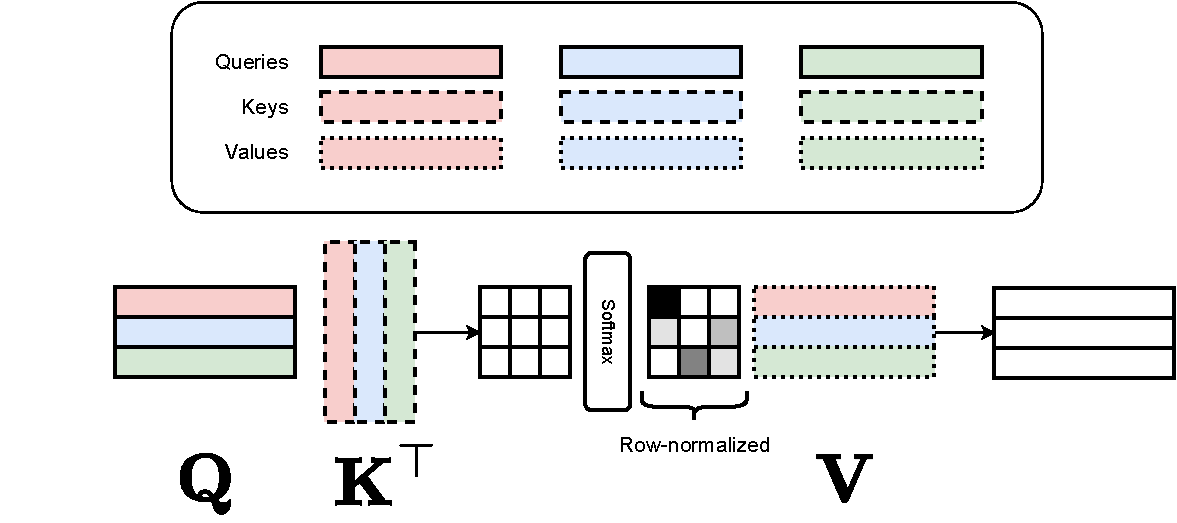
\includegraphics[width=0.9\textwidth]{images/attention-1}
    \caption{Visualization of the main operations of the SA layer (excluding projections).}
    \label{fig:self_attention}
\end{figure}


\subsection{Multi-head attention}
\label{subsec:multi_head_attention}

The previous layer is also called a \textbf{single-head} attention operation. It allows to model pairwise dependencies across tokens with high flexibility. However, in some cases we may have multiple sets of dependencies to consider: taking again the example of “\textit{the cat, which belongs to my mother, is on the table}”, the dependencies between “\textit{cat}” and “\textit{table}” are different with respect to the dependencies between “\textit{cat}” and “\textit{mother}”, and we may want the layer to be able to model them separately.\footnote{And everything depends on the cat, of course.}

A multi-head layer achieves this by running multiple attention operations in parallel, each with its own set of trainable parameters, before aggregating the results with some pooling operation. To this end, we define a new hyper-parameter $h$, that we call the number of \textbf{heads} of the layer. We instantiate $h$ separate projections for the tokens, for a total of $3hn$ tokens ($3n$ for each “head”):
%
\begin{align}\mathbf{K}_e=\mathbf{X}\mathbf{W}_{k,e} \\ 
\mathbf{V}_e=\mathbf{X}\mathbf{W}_{v,e} \\ 
\mathbf{Q}_e=\mathbf{X} \mathbf{W}_{q,e}
\end{align}
%
$\mathbf{W}_{k,e}$ represents the key projection for the $e$-th head, and similarly for the other quantities. The \textbf{multi-head attention} (MHA) layer performs $h$ separate SA operations, stacks the resulting output embeddings, and projects them a final time to the desired dimensionality:

\vspace{1em}
\begin{equation}
\text{MHA}(\mathbf{X})=\begin{bmatrix}\eqnmarkbox[drawred]{node}{\text{softmax}\left(\frac{\mathbf{Q}_1\mathbf{K}_1^\top}{\sqrt{k}}\right)\mathbf{V}_1} \;\mathbin\Vert\; \ldots \; \mathbin\Vert\;\text{softmax}\left(\frac{\mathbf{Q}_h\mathbf{K}_h^\top}{\sqrt{k}}\right)\mathbf{V}_h\end{bmatrix}\eqnmarkbox[drawgreen]{node2}{\mathbf{W}_o}
\label{eq:mha_explicit}
\end{equation}
\annotate[yshift=1em]{above,right}{node}{Individual SA layer}
\annotate[yshift=-1em]{below,left}{node2}{Output projection}

\vspace{0.5em}
Each SA operation returns a matrix of shape $(n,v)$. These $h$ matrices are concatenated across the second dimension to obtain a matrix $(n,hv)$, which is then projected with a matrix $\mathbf{W}_o \sim (o,hv)$, where $o$ is an additional hyper-parameter allowing flexibility in the choice of the output dimensionality.

\subsection*{An explanation of the terminology} 

In order to understand why the three tokens are called queries, keys, and values, \addteacup we consider the analogy of a SA layer with a standard Python dictionary, which is shown in Box \ref{code:dictionary}. 

\begin{mypy}{A dictionary in Python: a value is returned only if a perfect key-query match is found. Otherwise, we get an error.}{code:dictionary}
d = dict()
d["Simone"] = 2
d["Simone"]       # Returns 2
d["Smone "]       # Returns an error
\end{mypy}

Formally, a dictionary is a set of pairs of the form (key, value), where the key acts as an univocal ID to retrieve the corresponding value. For example, in the third and fourth line of Box \ref{code:dictionary} we query the dictionary with two different strings (“\textit{Simone}” and “\textit{Smone }”): the dictionary compares the query string to all keys which are stored inside, returning the corresponding value if a perfect match is found, an error otherwise.

Given a measure of similarity over pair of keys, we can consider a variant of a standard dictionary which always returns the value corresponding to the closest key found in the dictionary. If the keys, queries, and values are vectors, this dictionary variant is equivalent to our SA layer if we replace the softmax operation with an argmax over the tokens, as shown in Figure \ref{fig:hard_attention}.

This “hard” variant of attention is difficult to implement because the gradients of the argmax operation are zero almost everywhere (we will cover discrete sampling and approximating the argmax operation with a discrete relaxation in the next volume). Hence, we can interpret the SA layer as a soft approximation in which each token is updated with a weighted combination of all values based on the corresponding key/query similarities.

\begin{figure}[t]
    \centering
    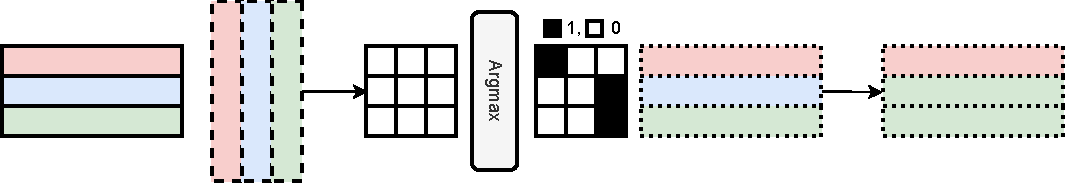
\includegraphics[width=1.0\textwidth]{images/attention-2}
    \caption{SA with a “hard” attention is equivalent to a vector-valued dictionary.}
    \label{fig:hard_attention}
\end{figure}

\begin{supportbox}{Heads and circuits}

We will see shortly that the MHA layer is always combined with a residual connection (Section \ref{sec:residual_connections}). In this case we can write its output for the $i$-th token as:

\vspace{2em}
\begin{equation}
\mathbf{x}_i \leftarrow \mathbf{x}_i + \eqnmarkbox[drawred]{node}{\sum_e} \eqnmarkbox[drawgreen]{node2}{\sum_j} \alpha_e(\mathbf{x}_i, \mathbf{x}_j)\mathbf{W}_e^\top \mathbf{x}_j
\end{equation}
\annotate[yshift=1em]{above,right}{node}{Sum over heads}
\annotate[yshift=-1em]{below,right}{node2}{Sum over tokens}

\vspace{2em}
where $\alpha_e(\mathbf{x}_i, \mathbf{x}_j)$ is the attention score between tokens $i$ and $j$ in head $e$, and $\mathbf{W}_e$ combines the value projection of the $e$-th head with the $e$-th block of the output projection in \eqref{eq:mha_explicit}. The token embeddings are sometimes called the \textbf{residual stream} of the model.\footnote{This has been popularized in the context of \textbf{mechanistic interpretability}, which tries to retro-engineer the layers' behaviour to find interpretable components called \textit{circuits}: \url{https://transformer-circuits.pub}. The linearity of the stream is fundamental for the analisys.} Hence, the heads can be understood as “reading” from the residual stream (via the projection by $\mathbf{W}_e$ and the selection via the attention scores), and linearly “writing” back on the streams.
\end{supportbox}

\section{Positional embeddings}
\label{sec:positional_embeddings}

With the MHA layer in hand, we consider the design of the complete transformer model, which requires another component, positional embeddings.

\subsection{Permutation equivariance of the MHA layer}

It is interesting to consider what happens to the output of a MHA layer when the order of the tokens is re-arranged (\textit{permuted}). To formalize this, we introduce the concept of \textbf{permutation matrices}.

\begin{definition}[Permutation matrix]
A \textbf{permutation matrix} of size $n$ is a square binary matrix $\mathbf{P} \sim \text{Binary}(n,n)$ such that only a single 1 is present on each row or column:

$$
\mathbf{1}^\top\mathbf{P}=\mathbf{1},\;\; \mathbf{P}\mathbf{1}=\mathbf{1}
$$

If we remove the requirement for the matrix to have binary entries and we only constrain the entries to be non-negative, we obtain the set of \textbf{doubly stochastic} matrices (matrices whose rows and columns sum to one).

\end{definition}

The effect of applying a permutation matrix is to rearrange the corresponding rows / columns of a matrix. For example, consider the following permutation:

$$
\mathbf{P}=\begin{bmatrix} 1 & 0 & 0 \\ 0 & 0 & 1 \\ 0 & 1 & 0 \end{bmatrix}
$$

Looking at the rows, we see that the second and third elements are swapped by its application:

$$
\mathbf{P}\begin{bmatrix} {\color{drawred}\mathbf{x}_1} \\ {\color{drawgreen}\mathbf{x}_2} \\ {\color{drawblue}\mathbf{x}_3} \end{bmatrix} = \begin{bmatrix} {\color{drawred}\mathbf{x}_1} \\ {\color{drawblue}\mathbf{x}_3}  \\ {\color{drawgreen}\mathbf{x}_2}\end{bmatrix}
$$

Interestingly, the only effect of applying a permutation matrix to the inputs of a MHA layer is to rearrange the outputs of the layer in an equivalent way:

$$
\text{MHA}(\mathbf{P}\mathbf{X})=\mathbf{P}\,\cdot\,\text{MHA}(\mathbf{X})
$$

\begin{figure}[t]
    \centering
    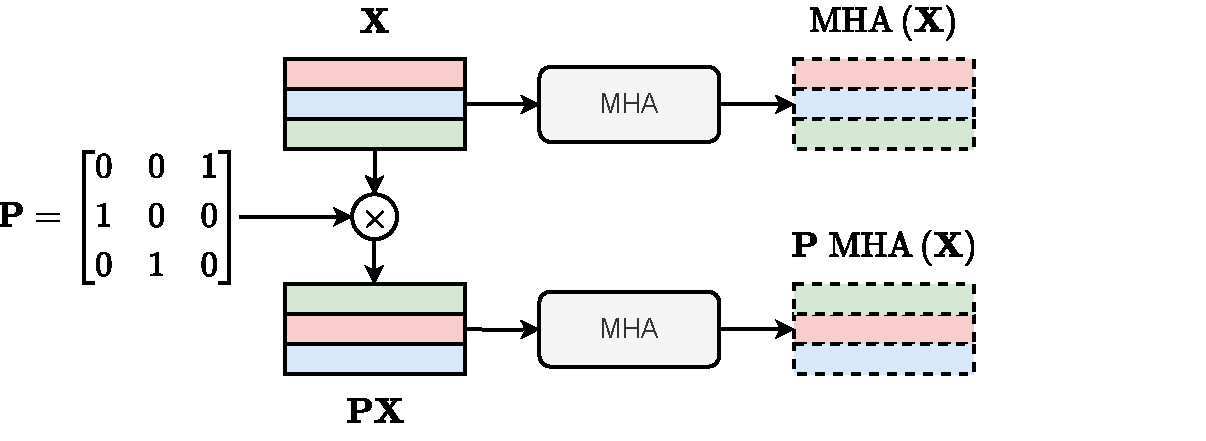
\includegraphics[width=0.95\textwidth]{images/permutation_equivariance}
    \caption{The output of a MHA layer after permuting the ordering of the tokens is trivially the permutation of the original outputs.}
    \label{fig:permutation_equivariance_mha}
\end{figure}

This is immediate to prove. We focus on the single headed variant as the multi-headed variant proceeds similarly. First, the softmax renormalizes the elements over the columns of a matrix, so it is trivially permutation equivariant across both rows and columns:

$$
\text{softmax}(\mathbf{P}\mathbf{X}\mathbf{P}^\top)=\mathbf{P}\left[\text{softmax}(\mathbf{X})\right]\mathbf{P}^\top
$$

From this we can immediately deduce the positional equivariance of SA:

\begin{gather}
\text{SA}(\mathbf{P}\mathbf{X}) = \text{softmax}\left(\mathbf{P}\frac{\mathbf{X}\mathbf{W}_q\mathbf{W}_k^\top\mathbf{X}^\top}{\sqrt{k}}\mathbf{P}^\top\right)\mathbf{P}\mathbf{X}\mathbf{W}_v \\ = \mathbf{P}\text{softmax}\left(\frac{\mathbf{X}\mathbf{W}_q\mathbf{W}_k^\top\mathbf{X}^\top}{\sqrt{k}}\right)\mathbf{X}\mathbf{W}_v = \mathbf{P}\cdot\text{SA}(\mathbf{X})
\end{gather}

where we make use of the fact that $\mathbf{P}^\top \mathbf{P} = \mathbf{I}$ for any permutation matrix. This can also be seen by reasoning on the SA layer for each token: the output is given by a sum of elements, each weighted by a pairwise comparison. Hence, for a given token the operation is \textbf{permutation invariant}. Instead, for the entire input matrix, the operation is \textbf{permutation equivariant}.

Translational equivariance was a desirable property for a convolutional layer, but permutation equivariance is \textit{undesirable} (at least here), because it discards the valuable ordering of the input sequence. As an example, the only effect of processing a text whose tokens have been reversed would be to reverse the output of the layer, despite the fact that the resulting reversed input is probably invalid. Formally, the SA and MHA layers are set functions, not sequence functions.

Instead of modifying the layer or adding layers that are not permutation equivariant, the transformer operates by introducing the new concept of \textbf{positional embeddings}, which are auxiliary tokens that depend only on the position of a token in a sequence (\textbf{absolute positional embeddings}) or the offset of two tokens (\textbf{relative positional embeddings}). We describe the two in turn.

\subsection{Absolute positional embeddings}

Each token in the input matrix $\mathbf{X} \sim (n,e)$ represents the \textit{content} of the specific piece of text (e.g., a subword). Suppose we fix the maximum length of any sequence to $m$ tokens. To overcome positional equivariance, we introduce an additional set of \textbf{positional embeddings} $\mathbf{S} \sim (m,e)$, where the vector $\mathbf{S}_i$ uniquely encodes the concept of “being in position $i$”. Hence, the sum of the input matrix with the first rows of $\mathbf{S}$:
%
$$
\mathbf{X}^\prime =  \mathbf{X} + \mathbf{S}_{1:n}
$$
%
is such that $\idx{\mathbf{X}^\prime}{i}$ represents “token $\mathbf{X}_i$ in position $i$”.
%
Because it does not make sense to permute the positional embeddings (as they only depend on the position), the resulting layer is not permutation equivariant anymore:
%
$$
\text{MHA}(\mathbf{P}\mathbf{X} + \mathbf{S}) \neq \mathbf{P}\,\cdot\,\text{MHA}(\mathbf{X}+\mathbf{S})
$$
%
See Figure \ref{fig:positional_embeddings} for a visualization of this idea. 

\begin{SCfigure}[1.5]
    \centering
    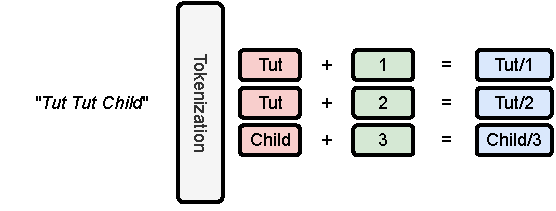
\includegraphics[width=0.6\textwidth]{images/positional_embeddings}
    \caption{Positional embeddings (\colorbox{drawgreen!30}{green}) added to the  tokens' embeddings (\colorbox{drawred!30}{red}). The same token in different positions has different outputs (\colorbox{drawblue!30}{blue}).}
    \label{fig:positional_embeddings}
\end{SCfigure}

How should we build positional embeddings? The easiest strategy is to consider $\mathbf{S}$ as part of the model's parameters, and train it together with the rest of the trainable parameters, similarly to the token embeddings. This strategy works well  when the number of tokens is relatively stable; we will see an example in the next chapter in the context of computer vision.

Alternatively, we can define some deterministic function from the set of tokens' positions to a given vector that uniquely identifies the position. Some strategies are clearly poor choices, for example:
%
\begin{enumerate}
\item We can associate to each position a scalar $p=i/m$ which is linearly increasing with the position. However, adding a single scalar to the token embeddings has a minor effect.
\item We can one-hot encode the position into a binary vector of size $m$, but the resulting vector would be extremely sparse and high-dimensional.
\end{enumerate}
%
A possibility, introduced in the original transformer paper \cite{vaswani2017attention}, is that of \textbf{sinusoidal embeddings}. To understand them, consider a sine function:
%
$$
y=\sin(x)
$$
%
The sine assigns a unique value to any input $x$ inside the range $[0, 2\pi]$. We can also vary the frequency of the sine:
%
$$
y=\sin(\omega x)
$$
%
This oscillates more or less rapidly based on the frequency $\omega$, and it assigns a unique value to any input in the range $[0, \frac{2\pi}{\omega}]$. There is an analogy with an (analogical) clock: the seconds' hand makes a full rotation with a frequency of $\frac{1}{60}$ Hz (once every minute). Hence, every “point in time” inside a minute can be distinguished by looking at the hand, but two time instants in general can only be identified modulo 60 seconds. We overcome this in a clock by adding a separate hand (the minute hand) that rotates with a much slower frequency of $\frac{1}{3600}$ Hz. Hence, by looking at the pair of coordinates (second, minute) (the “embedding” of time) we can distinguish any point inside an hour. Adding yet another hand with an even slower frequency (the hour hand) we can distinguish any point inside a day. This can be generalized: we could design clocks with lower or higher frequencies to distinguish months, years, or milliseconds.

A similar strategy can be applied here: we can distinguish each position $i$ by encoding it through a set of $e$ sines (with $e$ an hyper-parameter) of increasing frequencies:
%
$$
\mathbf{S}_i=\left[ \sin(\omega_1i), \sin(\omega_2i),\ldots,\sin(\omega_ei) \right]
$$
%
In practice, the original proposal from \cite{vaswani2017attention} uses only $e/2$ possible frequencies, but adds both sines and cosines:
%
$$
\mathbf{S}_i=\left[ \sin(\omega_1i), \cos(\omega_1i),\sin(\omega_2i), \cos(\omega_2i),\ldots,\sin(\omega_{e/2}i), \cos(\omega_{e/2}i) \right]
$$
%
This can be justified by noting that in this embedding, two positions are related via a simple linear transformation, a rotation, that depends only on the relative offset of the two positions.\footnote{See \url{https://kazemnejad.com/blog/transformer_architecture_positional_encoding/} for a worked-out computation.} Any choice of frequency is valid provided they are sufficiently large and increasing at a super-linear rate. The choice from \cite{vaswani2017attention} was a geometric progression:
%
$$
\omega_i=\frac{1}{10000^{i/e}}
$$
%
that varies from $\omega_0=1$ to $\omega_e=\frac{1}{10000}$. See Figure \ref{fig:positional_embeddings_plot} for a visualization.

\begin{SCfigure}
    \centering
    \hspace{1em}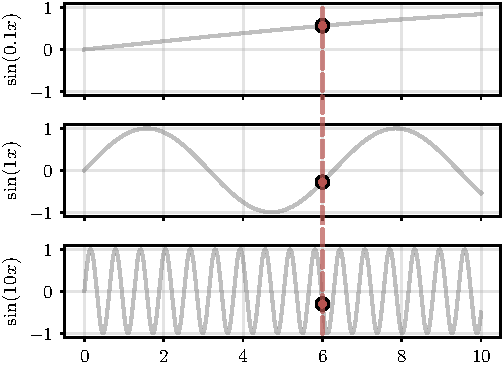
\includegraphics[width=0.6\textwidth]{images/positional_embeddings_plot}
    \caption{We show three $\sin$ functions with $\omega=0.1$, $\omega=1$, and $\omega=10$. The embedding for position $x=6$ is given by the corresponding values (red circles).}
    \label{fig:positional_embeddings_plot}
\end{SCfigure}

\subsection{Relative positional embeddings}

Trainable positional embeddings and sinuisodal positional embeddings are examples of \textbf{absolute} embeddings, because they encode a specific position in the sequence. An alternative that has become common with very long sequences are \textbf{relative positional embeddings}. In this case, instead of adding a positional encoding to a token, we modify the attention function to make it dependent on the offset between any two tokens:
%
$$
g(\mathbf{x}_i, \mathbf{x}_j)\rightarrow g(\mathbf{x}_i, \mathbf{x}_j, i-j)
$$
%
This is a combination of the two ideas we introduced at the beginning of this chapter (Figure \ref{fig:biases}). Note that while absolute embeddings are added only once (at the input), relative embeddings must be added every time an MHA layer is used. As an example, we can add a trainable bias matrix $\mathbf{B} \sim (m,m)$ and rewrite the dot product with an offset-dependent bias:
%
$$
g(\mathbf{x}_i,\mathbf{x}_j)=\mathbf{x}_i^\top\mathbf{x}_j+B_{ij}
$$
%
A simpler variant, \textbf{attention with linear biases} (ALiBi) \cite{press2021train}, considers a single trainable scalar in each head which is multiplied by a matrix of offsets. More advanced strategies, such as \textbf{rotary positional embeddings} (RoPE), are also possible \cite{su2024roformer}.

\section{Building the transformer model}
\subsection{The transformer block and model}
\label{subsec:transformer_block}

A model could be built, in principle, from a stack of multiple MHA layers (with the softmax providing the non-linearity necessary to avoid the collapse of multiple linear projections). Empirically, however, it is found that the MHA works best when interleaved with a separate fully-connected block that operates on each token independently. These two operations can be understood as mixing the tokens (MHA), and mixing the channels (MLP), similarly to the depthwise-separable convolution  model.

In particular, for the MLP block it is common to choose a bottleneck architecture composed of two fully-connected layers of the form:
%
$$
\text{MLP}(\mathbf{x})=\mathbf{W}_2\phi\left(\mathbf{W}_1\mathbf{x}\right)
$$
%
where $\mathbf{x} \sim (e)$ is a token, $\mathbf{W}_1 \sim (p, e)$, with $p$ selected as an integer multiple of $e$ (e.g., $p=3e$ or $p=4e$), and $\mathbf{W}_2 \sim (e,p)$ reprojecting back to the original embedding dimension. Biases are generally removed as the increased hidden dimension provides sufficient degrees of freedom.

To ensure efficient training of deep models we also need a few additional regularization strategies. In particular, it is common to include two layer normalization steps and two residual connections, respectively for the MHA and MLP blocks. Depending on where the layer normalization is applied, we obtain two variants of the basic transformer block, sometimes denoted as \textbf{pre-normalized} and \textbf{post-normalized}. These are shown in Figure \ref{fig:pre_post_normalization}.

\begin{SCfigure}
    \centering
    \hspace{2em}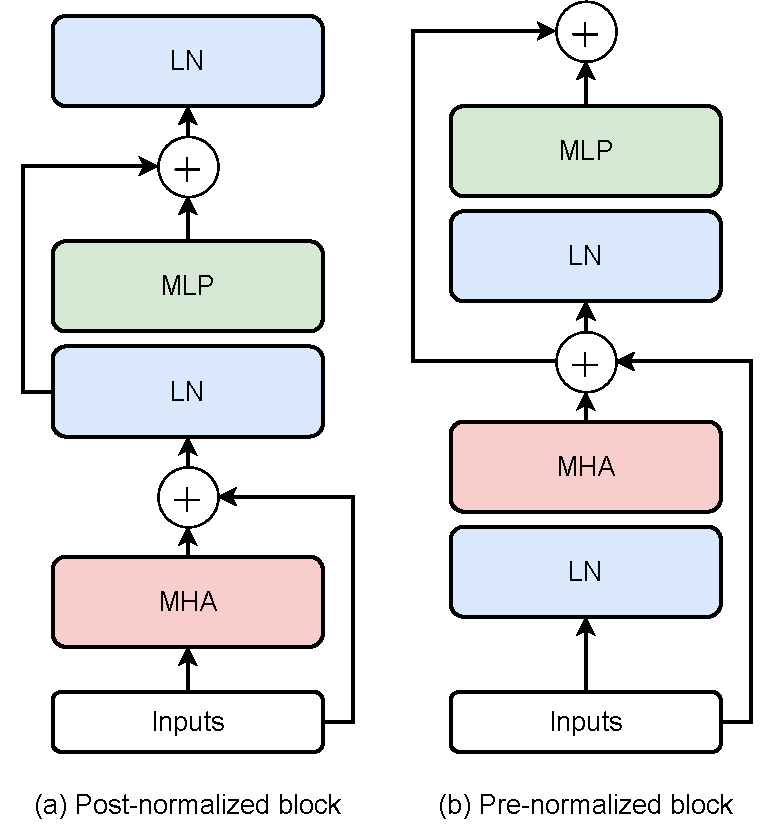
\includegraphics[width=0.4\textwidth]{images/transformer_block}
    \caption{Schematic view of pre-normalized and post-normalized transformer blocks. In the post-normalized variant the LN block is applied after the MHA or MLP operation, while in the pre-normalized one before each layer.}
    \label{fig:pre_post_normalization}
\end{SCfigure}

While the post-normalized version corresponds to the original transformer block, the pre-normalized variant is generally found to be more stable and faster to train \cite{xiong2020layer}. The design of the block in Figure \ref{fig:pre_post_normalization} is, fundamentally, an empirical choice, and many variants have been proposed and tested in the literature. We review some of these later on in Section \ref{subsec:mha_variants}.

We can now complete the description of a basic transformer model:
%
\begin{enumerate}
\item Tokenize and embed the original input sequence in a matrix $\mathbf{X} \sim (n,e)$.\
\item If using absolute positional embeddings, add them to the input matrix.
\item Apply 1 or more blocks of the form discussed above.
\item Include a final head depending on the task.
\end{enumerate}
%
The output of step (3) is a set of processed tokens $\mathbf{H} \sim (n,e)$, where neither $n$ nor $e$ are changed by the transformer model (the former because we do not have local pooling operations on sets, the latter because of the residual connections in the block). Considering for example a classification task, we can apply a standard classification head by pooling over the tokens and proceeding with a fully-connected block:
%
$$
y=\text{softmax}\left(\text{MLP}\left(\frac{1}{n}\sum_i\mathbf{H}_i\right)\right)
$$
%
This part is identical to its corresponding CNN design. However, the transformer has a number of interesting properties, mostly stemming by the fact that it manipulates its input as a set, without modifying its dimensionality throughout the architecture. We investigate one simple example next.

\subsection{Class tokens and register tokens}
\label{subsec:class_register_tokens}

While up to now we have assumed that each token corresponds to one part of our input sequence, nothing prevents us from adding \textit{additional} tokens to the input of the transformer. This is strictly dependent on its specific architecture: a CNN, for example, requires its input to be precisely ordered, and it is not clear how we could add additional tokens to an image or to a sequence. This is a very powerful idea, and we only consider two specific implementations here.

First, we consider the use of a \textbf{class token} \cite{dosovitskiy2020image}, an additional token which is added explicitly for classification in order to replace the global pooling operation above. Suppose we initialize a single trainable token $\mathbf{c} \sim (e)$, which is added to the input matrix:
%
$$
\mathbf{X} \leftarrow\begin{bmatrix}\mathbf{X} \\ \mathbf{c}^\top \end{bmatrix}
$$
%
The new matrix has shape $(n+1, e)$. The class token is identical for all sequences in a mini-batch. After step (3) above, the transformer outputs a matrix $\mathbf{H} \sim (n+1,e)$ of updated representations for all tokens, including the class one. The idea is that, instead of pooling over the tokens, the model should be able to “compress” all information related to the classification task inside the class token, and we can rewrite the classification head by simply discarding all other tokens:\footnote{In the language of circuits and heads from Section \ref{subsec:multi_head_attention}, we could say equivalently that the model must learn to move all information related to the classification in the residual stream of the class token.}
%
$$
y=\text{softmax}\left(\text{MLP}\left(\mathbf{H}_{n+1}\right)\right)
$$
%
Additional trainable tokens can be useful even if not explicitly used. For example, \cite{darcet2023vision} has shown that adding a few additional tokens (called \textbf{registers} in this case) can improve the quality of the attention maps by providing the model with the possibility of using the registers to “store” auxiliary information that does not depend explicitly on a given position.

\section*{From theory to practice}

\begin{wrapfigure}{r}{3.0cm}
\vspace{-6em}
\includegraphics[width=3.0cm]{images/shutterstock_2075221579.jpg}
\vspace{-4em}
\end{wrapfigure}

We will introduce many important concepts related to transformers in the next chapter. Thus, for this chapter I am suggesting a slightly unconventional exercise which combines a convolutional backbone with a transformer-like head -- as depicted in Figure \ref{fig:multiview_model}.

\begin{figure}[t]
    \centering
    \hspace{1em}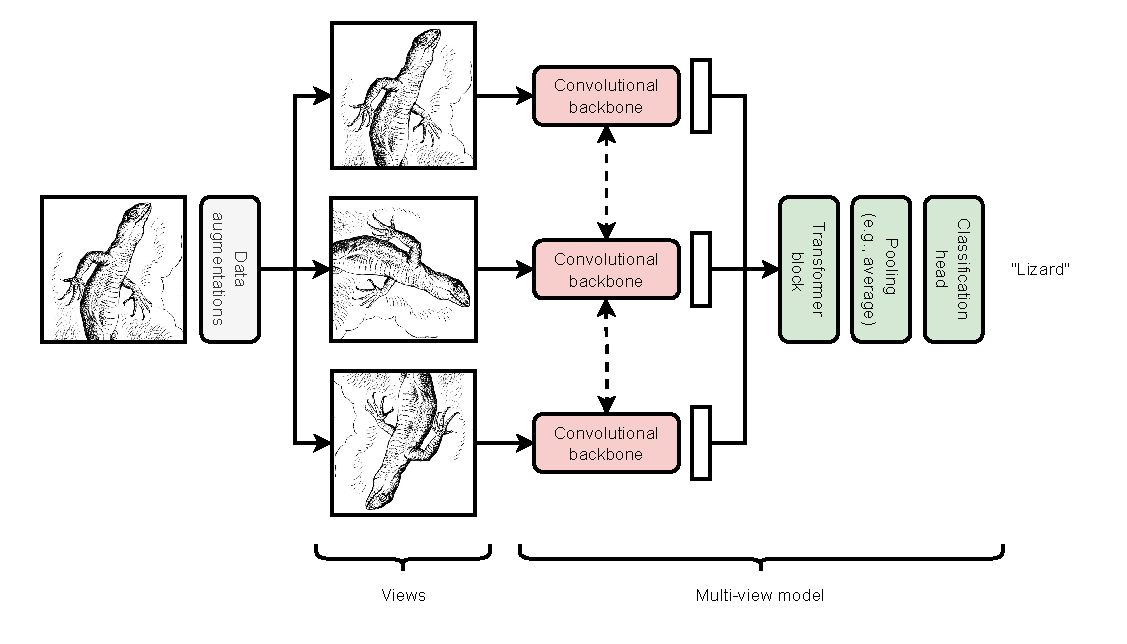
\includegraphics[width=1\textwidth]{images/Multiviewmodel}
    \caption{Multi-view model to be implemented in this chapter. The image is augmented through a set of random data augmentation strategies to obtain a set of \textbf{views} of the input (\colorbox{gray!30}{gray}). Each \textit{view} is processed by the same convolutional backbone to obtain a fixed-sized dimensional embedding (\colorbox{drawred!30}{red}). The set of embeddings are processed by a transformer block before the final classification (\colorbox{drawgreen!30}{green}). Illustration by John Tenniel.}
    \label{fig:multiview_model}
\end{figure}

The convolutional models you developed in Chapters \ref{chap:cnns} and \ref{chap:deep_cnns} were applied to a \textit{single} image. However, sometimes we have available a \textit{set} of images of the same object to be recognized -- for example, in a monitoring system, we may have multiple screenshots of a suspicious person. This is called a \textbf{multi-view} system in the literature, and each image is called a \textbf{view} of the object. A multi-view model should provide a single prediction for the entire set of views, while being invariant to the order of the views in input. For this exercise we will implement a simple multi-view model -- see Figure \ref{fig:multiview_model}.

\begin{enumerate}
\item Using any image classification dataset, you can simulate a multi-view model by applying a fixed number of data transformations to the input (gray block in Figure \ref{fig:multiview_model}). Ignoring the batch dimension, for each input image of shape $x \sim (h,w,c)$ (height, width, channels), you obtain a \textit{multi-view} input of shape $x^\prime \sim (v,h,w,c)$, where $v$ is the number of views. A single label $y$ is associated to this tensor -- the label of the original image. The number of views can also be different from mini-batch to mini-batch, as no part of the model is constrained to a pre-specified number of view.
\item The multi-view model is composed of three components. Denote by $g(x)$ a model that processes a single view to a fixed-dimensional embedding -- for example, this can be any convolutional backbone you trained for the previous exercises. The first part of the full model (red part in Figure \ref{fig:multiview_model}) applies $g$ in parallel to all views, $\mathbf{h}_i = g(x_i) \sim (e)$, where $e$ is a hyper-parameter (the output size of the backbone).
\item After concatenating the embeddings of the views we obtain a matrix $\mathbf{H} \sim (v, e)$. In order for the full model to be permutation invariant, any component applied on $\mathbf{H}$ must be permutation equivariant.\footnote{An average operation over the views is the simplest example of permutation invariant layer. Hence, removing the MHA block from Figure \ref{fig:multiview_model} is also a valid baseline. Alternatively, deep sets \cite{zaheer2017deep} characterize the full spectrum of linear, permutation invariant layers.} For the purposes of this exercise, implement and apply a single transformer block as per Section \ref{subsec:transformer_block}. You can implement MHA using basic PyTorch, or you can try a more advanced implementation using \texttt{einops}.\footnote{See \url{https://einops.rocks/pytorch-examples.html}.} You can also compare with the pre-implemented version in \mintinline{python}{torch.nn}.
\item The transformer block does not modify the input shape. To complete the model, perform an average over the views (which represent the tokens in this scenario), and apply a final classification head. You can also experiment with adding a class token (Section \ref{subsec:class_register_tokens}). It is easy to show that a model built in this way is permutation invariant with respect to the views.
\end{enumerate}